\section{Introduction}

Relation extraction (RE) \cite{Bach} is an important and open 
research task in the branch of information extraction (IE) \cite{Grishman1997}.
RE task aims at extracting instances of specific relation types from natural language sentences.
The target relation type $r$ is usually binary relation, 
thus the result of RE is formed of ($e_1$, $r$, $e_2$) triples,
where the relation argument $e_1$ and $e_2$ are named entities extracted from sentences.
%between entities
%from a natural language sentence.
%When the target relation is binary, the result of RE is in the form of ($e_1$, $r$, $e_2$) 
%triples.
\figref{fig:intro} illustrates the RE task.
The example sentence contains 4 named entities with 2 relation types,
and we can extract two relation triples, named
(``Tim Cook'', \textit{LeaderOf}, ``Apple'') and (``Beijing'' \textit{CityOf}, ``China'').
%One of the relation arguments triples is \{Tim Cook, LeaderOf, Apple\},  where $e_1$ is a person entity 
%``Tim Cook'', $r$ is ``LeaderOf'', and $e_2$ is ``Apple''.
\begin{figure}[th]
  \centering
  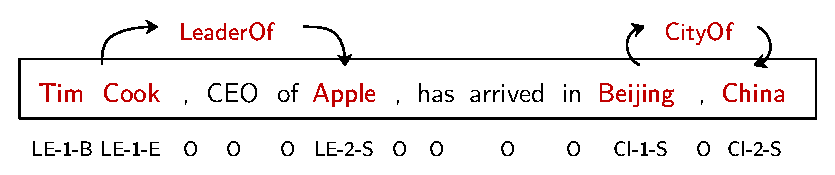
\includegraphics[width=\columnwidth]{pictures/introduction.eps}
  \caption{An example of relation extraction and RE tagging scheme.}
  \label{fig:intro}
\end{figure}

RE is a challenging task and still far from being solved due to the 
variety and ambiguity of natural language. 
Traditional methods regard the RE task as a pipeline of two sub-tasks:
named entity recognition (NER) \cite{zhou2002named,Nadeau2007,Dernoncourt2017} and 
relation classification (RC)
\cite{Zeng2014,Wang2016,Wen2017,Cai2016,Zhou2016,Xu2015}. 
%Traditionally, the problem of RE has been treated as a sequence of two
%sub-tasks, namely named entity recognition (NER) \cite{Nadeau2007} and relation
%classification (RC) \cite{Zeng2014}.
%Solving RE amounts to first recognizing the
%named entities in the sentence, and then determining the relation type
%between these entities. 
As a cascading approach, the NER task recognizes named entities (NE)
within the sentence, then RC task performs classification for each extracted NE pair.
%determining the relation type between all tagged entity pairs.
%The latter sub-task of RE depends on the result of NER. 
%In the past, the most successful approaches to solve RE come from
%machine learning and they fall into two categories, pipelined
%\cite{Zeng2014,Wang2016,Wen2017,Cai2016,Zhou2016,Xu2015}
%and joint approaches
%\cite{Zheng2017a,Li2017a,Li2014,Adel2017,Gupta2016,Miwa2014,Kate2010,
%  Miwa2016,Katiyar2017,Ren2017}. Pipelined approaches treat NER and RC as two
%separate tasks and trains two independent models. The obvious
%drawback of this approach is that the training of NER or RC cannot benefit
%each other, when in reality the two sub-tasks are inter-dependent \YY{Need a
%  reference}. This inspires the second category of approaches which train the
%two models jointly by sharing some common, low-level parameters. 
%This type of joint-learning
%showed some advantage against the first approach and gained popularity lately.
%However, the joint approaches still produce two models and they
%are used sequentially at prediction time. 
The biggest disadvantage of such a two-step RE approach is error propagation
from NER to RC, since the performance of the second task highly relies on 
the result of the first task, while no feedback is available.

\begin{figure}[th]
\centering
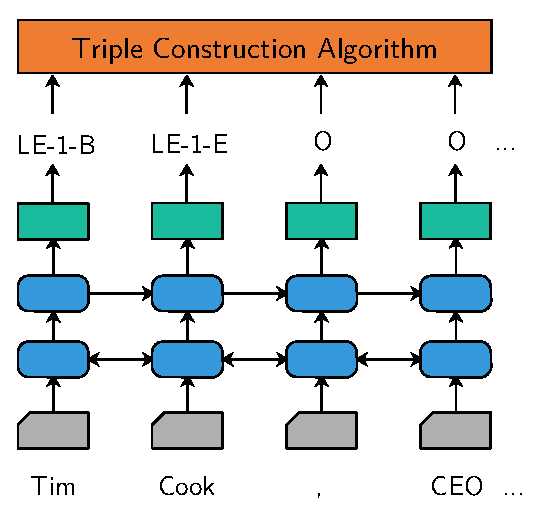
\includegraphics[width=4.5cm]{pictures/model.eps}
\caption{Sequential tagging model for relation extraction \cite{Zheng2017}. \label{fig:model}}
\end{figure}

To address the challenge, Zheng et al. \shortcite{Zheng2017} proposes a new approach,
which combines NER and RC into a single sequential labeling task by a novel
tagging scheme (see \figref{fig:model}).
In this new approach, each word in the sentence is labeled with a special tag,
containing both named entity and relation type information, as illustrated in
\figref{fig:intro}. For example, the tag for ``Tim'' is 
``LE-1-B'', where ``LE'' is the abbreviation of \textit{LeaderOf}, 
``1'' means both ``Tim'' is  $e_1$ of \textit{LeaderOf} relation, 
``B'' means ``Tim'' is the beginning of this entity.
In this framework, RNN is used to output the RE tags. 
The input is word sequence of a sentence. After the word
embedding layer, a BiLSTM is used to extract low level features. Then a forward
LSTM and a softmax layer is used to decode the tag sequence. 

After labeling a sentence, the predicted tagging sequences can be converted into 
the final relation triples ($e_1$, $r$, $e_2$) through triple 
construction algorithms. Zheng et al. \shortcite{Zheng2017} presented a naive
and less intuitive
algorithm for triple construction, but still achieved state-of-the-art result on
the popular NYT relation extraction dataset~\cite{Ren2017}.
%In this paper, We focus on the triple construction algorithm,
%there still have rooms for improvement.
%To address the challenge, Zheng et al.~\shortcite{Zheng2017}
%proposed to view RE as a normal sequence tagging problem and
%thus do away with the two sequential sub-tasks. 
%This new approach infers for each word in a
%sentence a special tag that contains both entity and relation information. 
%Once the words in a sentence is tagged, we can then reconstruct relation triples.
%While this idea is great, Zheng et al. only presented a very simple and hardly
%intuitive algorithm for triple construction.
%rooms for improvement.

In this paper, we evaluate several heuristic algorithms to construct relation
triples from tag sequences. Note that this problem setting does not take relation
overlapping into consideration. We perform experiments on the NYT benchmark dataset.
The experimental results show that these proposed algorithms
significantly outperform the previous ones, and one of them can achieve up to
7\% improvement over state-of-the-art results in F1.

